% =============================================================================
% Chapter 3: Tokenization
% =============================================================================
\chapter{Tokenization}
\label{ch:tokenization}

\begin{objectives}
    \item Understand why tokenization is necessary
    \item Learn how Byte Pair Encoding (BPE) works
    \item Train a tokenizer on real data
    \item Encode and decode text
    \item Understand special tokens and their purposes
\end{objectives}

% -----------------------------------------------------------------------------
\section{Why Tokenization?}
% -----------------------------------------------------------------------------

Neural networks operate on numbers, not text. Before we can feed text into a language model, we need to convert it into a sequence of integers. This process is called \textbf{tokenization}.

\begin{definition}[title=Tokenization]
\textbf{Tokenization} is the process of breaking text into discrete units (tokens) and mapping each unit to a unique integer ID.
\end{definition}

But how should we split text? There are several approaches, each with tradeoffs.

\subsection{Character-Level Tokenization}

The simplest approach: treat each character as a token.

\begin{lstlisting}[style=python]
text = "Hello"
tokens = list(text)  # ['H', 'e', 'l', 'l', 'o']
\end{lstlisting}

\textbf{Pros:}
\begin{itemize}
    \item Small vocabulary (just 256 bytes or ~65k Unicode characters)
    \item Can represent any text
\end{itemize}

\textbf{Cons:}
\begin{itemize}
    \item Very long sequences (``Hello'' becomes 5 tokens)
    \item Hard for the model to learn word-level patterns
\end{itemize}

\subsection{Word-Level Tokenization}

Split on whitespace and punctuation.

\begin{lstlisting}[style=python]
text = "Hello, world!"
tokens = ["Hello", ",", "world", "!"]
\end{lstlisting}

\textbf{Pros:}
\begin{itemize}
    \item Linguistically meaningful units
    \item Shorter sequences
\end{itemize}

\textbf{Cons:}
\begin{itemize}
    \item Huge vocabulary needed (English has 170k+ words)
    \item Cannot handle unknown words
    \item Doesn't work well across languages
\end{itemize}

\subsection{Subword Tokenization: The Best of Both Worlds}

Modern language models use \textbf{subword tokenization}, which splits text into units smaller than words but larger than characters.

\begin{lstlisting}[style=python]
text = "unhappiness"
tokens = ["un", "happiness"]  # or ["un", "happ", "iness"]
\end{lstlisting}

\begin{keypoint}
Subword tokenization balances vocabulary size with sequence length. Common words are single tokens; rare words are split into frequent subwords.
\end{keypoint}

\TryLM uses \textbf{Byte Pair Encoding (BPE)}, the most popular subword tokenization algorithm.

% -----------------------------------------------------------------------------
\section{Byte Pair Encoding (BPE)}
% -----------------------------------------------------------------------------

BPE was originally a data compression algorithm, adapted for NLP by Sennrich et al. (2016). It works by iteratively merging the most frequent pairs of tokens.

\subsection{The BPE Algorithm}

\begin{algorithm}[H]
\caption{Byte Pair Encoding Training}
\begin{algorithmic}[1]
\Require Training corpus, vocabulary size $V$
\State Initialize vocabulary with all individual bytes/characters
\While{vocabulary size $< V$}
    \State Count frequency of all adjacent token pairs in corpus
    \State Find the most frequent pair $(a, b)$
    \State Create new token $ab$ by merging $a$ and $b$
    \State Add $ab$ to vocabulary
    \State Replace all occurrences of $(a, b)$ with $ab$ in corpus
\EndWhile
\State \Return vocabulary and merge rules
\end{algorithmic}
\end{algorithm}

\subsection{BPE Example}

Let's trace through BPE on a toy corpus:

\begin{lstlisting}[style=shell, numbers=none]
Corpus: "low lower lowest"
Initial tokens: ['l', 'o', 'w', ' ', 'l', 'o', 'w', 'e', 'r', ' ',
                 'l', 'o', 'w', 'e', 's', 't']
\end{lstlisting}

\textbf{Iteration 1:} Most frequent pair is `(l, o)` (3 occurrences)
\begin{lstlisting}[style=shell, numbers=none]
Merge: l + o -> lo
Tokens: ['lo', 'w', ' ', 'lo', 'w', 'e', 'r', ' ', 'lo', 'w', 'e', 's', 't']
\end{lstlisting}

\textbf{Iteration 2:} Most frequent pair is `(lo, w)` (3 occurrences)
\begin{lstlisting}[style=shell, numbers=none]
Merge: lo + w -> low
Tokens: ['low', ' ', 'low', 'e', 'r', ' ', 'low', 'e', 's', 't']
\end{lstlisting}

\textbf{Iteration 3:} Most frequent pair is `(low, e)` (2 occurrences)
\begin{lstlisting}[style=shell, numbers=none]
Merge: low + e -> lowe
Tokens: ['low', ' ', 'lowe', 'r', ' ', 'lowe', 's', 't']
\end{lstlisting}

The algorithm continues until reaching the target vocabulary size.

\begin{figure}[H]
\centering
\begin{tikzpicture}[
    box/.style={rectangle, draw, minimum width=0.8cm, minimum height=0.6cm, font=\ttfamily\small},
    merge/.style={-{Stealth}, thick, red!70!black},
]
    % Initial
    \node at (-2, 0) {\textbf{Initial:}};
    \foreach \x/\c in {0/l, 0.9/o, 1.8/w, 2.7/e, 3.6/r} {
        \node[box, fill=blue!10] at (\x, 0) {\c};
    }

    % After merge 1
    \node at (-2, -1.2) {\textbf{Merge 1:}};
    \node[box, fill=green!20, minimum width=1.6cm] at (0.45, -1.2) {lo};
    \foreach \x/\c in {1.8/w, 2.7/e, 3.6/r} {
        \node[box, fill=blue!10] at (\x, -1.2) {\c};
    }
    \draw[merge] (0, -0.4) -- (0.2, -0.8);
    \draw[merge] (0.9, -0.4) -- (0.7, -0.8);

    % After merge 2
    \node at (-2, -2.4) {\textbf{Merge 2:}};
    \node[box, fill=green!20, minimum width=2.4cm] at (0.9, -2.4) {low};
    \foreach \x/\c in {2.7/e, 3.6/r} {
        \node[box, fill=blue!10] at (\x, -2.4) {\c};
    }

    % After merge 3
    \node at (-2, -3.6) {\textbf{Merge 3:}};
    \node[box, fill=green!20, minimum width=3.2cm] at (1.35, -3.6) {lowe};
    \node[box, fill=blue!10] at (3.6, -3.6) {r};
\end{tikzpicture}
\caption{BPE merge process for the word ``lower''}
\label{fig:bpe-merges}
\end{figure}

\subsection{Byte-Level BPE}

\TryLM uses \textbf{byte-level BPE}, which operates on raw bytes rather than characters. This has important advantages:

\begin{itemize}
    \item \textbf{Universal}: Can tokenize any text in any language
    \item \textbf{No unknown tokens}: Every byte sequence can be represented
    \item \textbf{Compact base vocabulary}: Only 256 base tokens (one per byte)
\end{itemize}

% -----------------------------------------------------------------------------
\section{Special Tokens}
% -----------------------------------------------------------------------------

Beyond regular text tokens, we need special tokens to mark important positions in sequences.

\subsection{The Four Special Tokens}

\TryLM uses four special tokens:

\begin{table}[H]
\centering
\begin{tabular}{lll}
\toprule
\textbf{Token} & \textbf{Name} & \textbf{Purpose} \\
\midrule
\texttt{<|bos|>} & Beginning of Sequence & Marks the start of a text \\
\texttt{<|eos|>} & End of Sequence & Marks the end of a text \\
\texttt{<|pad|>} & Padding & Fills unused positions in batches \\
\texttt{<|unk|>} & Unknown & Represents unknown tokens (rarely used) \\
\bottomrule
\end{tabular}
\caption{Special tokens in TryLM}
\label{tab:special-tokens}
\end{table}

\subsection{Why Special Tokens?}

\textbf{BOS (Beginning of Sequence):} Tells the model ``a new sequence is starting.'' During generation, we start with BOS and let the model predict what follows.

\textbf{EOS (End of Sequence):} Tells the model ``this sequence is complete.'' During generation, when the model outputs EOS, we stop generating.

\textbf{PAD (Padding):} When batching sequences of different lengths, we pad shorter ones to match the longest. PAD tokens are ignored during training.

\begin{figure}[H]
\centering
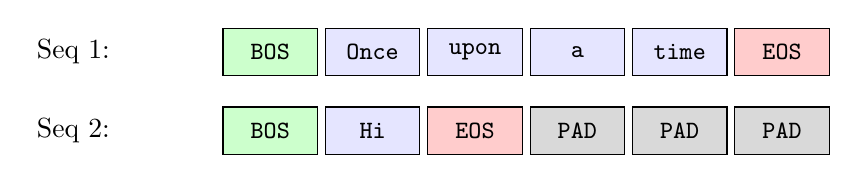
\begin{tikzpicture}[
    box/.style={rectangle, draw, minimum width=1.2cm, minimum height=0.6cm, font=\ttfamily\small},
]
    % Sequence 1
    \node at (-2.5, 0) {Seq 1:};
    \node[box, fill=green!20] at (0, 0) {BOS};
    \node[box, fill=blue!10] at (1.3, 0) {Once};
    \node[box, fill=blue!10] at (2.6, 0) {upon};
    \node[box, fill=blue!10] at (3.9, 0) {a};
    \node[box, fill=blue!10] at (5.2, 0) {time};
    \node[box, fill=red!20] at (6.5, 0) {EOS};

    % Sequence 2 (shorter, padded)
    \node at (-2.5, -1) {Seq 2:};
    \node[box, fill=green!20] at (0, -1) {BOS};
    \node[box, fill=blue!10] at (1.3, -1) {Hi};
    \node[box, fill=red!20] at (2.6, -1) {EOS};
    \node[box, fill=gray!30] at (3.9, -1) {PAD};
    \node[box, fill=gray!30] at (5.2, -1) {PAD};
    \node[box, fill=gray!30] at (6.5, -1) {PAD};
\end{tikzpicture}
\caption{Two sequences in a batch with padding}
\label{fig:special-tokens}
\end{figure}

% -----------------------------------------------------------------------------
\section{The TryLM Tokenizer}
% -----------------------------------------------------------------------------

Now let's look at how \TryLM implements tokenization. The tokenizer is built on the HuggingFace \texttt{tokenizers} library.

\subsection{Tokenizer Architecture}

\begin{lstlisting}[style=python, caption={Tokenizer training from tokenizer.py}]
@classmethod
def train(
    cls,
    texts: Iterator[str],
    config: TokenizerConfig,
    show_progress: bool = True,
) -> "TryLMTokenizer":
    """Train a new BPE tokenizer on the given texts."""
    # Initialize BPE tokenizer
    tokenizer = Tokenizer(models.BPE(unk_token=config.unk_token))

    # Set up pre-tokenization (GPT-2 style byte-level)
    tokenizer.pre_tokenizer = pre_tokenizers.ByteLevel(
        add_prefix_space=False
    )

    # Set up decoder
    tokenizer.decoder = decoders.ByteLevel()

    # Configure trainer
    trainer = trainers.BpeTrainer(
        vocab_size=config.vocab_size,
        min_frequency=config.min_frequency,
        special_tokens=config.special_tokens,
        show_progress=show_progress,
    )

    # Train the tokenizer
    tokenizer.train_from_iterator(texts, trainer=trainer)

    return cls(tokenizer, config)
\end{lstlisting}

\subsection{Key Components}

\begin{enumerate}
    \item \textbf{Model}: \texttt{BPE} --- the core tokenization algorithm
    \item \textbf{Pre-tokenizer}: \texttt{ByteLevel} --- converts text to bytes before BPE
    \item \textbf{Decoder}: \texttt{ByteLevel} --- converts bytes back to text
    \item \textbf{Trainer}: \texttt{BpeTrainer} --- learns the merge rules from data
\end{enumerate}

\subsection{Post-Processing}

After tokenization, we add special tokens automatically:

\begin{lstlisting}[style=python]
# Set up post-processor to add BOS/EOS tokens
tokenizer.post_processor = TemplateProcessing(
    single=f"{config.bos_token}:0 $A:0 {config.eos_token}:0",
    special_tokens=[
        (config.bos_token, bos_id),
        (config.eos_token, eos_id),
    ],
)
\end{lstlisting}

This means every encoded sequence automatically gets BOS at the start and EOS at the end:

\begin{lstlisting}[style=shell, numbers=none]
Input:  "Hello world"
Output: [<|bos|>, Hello, world, <|eos|>]
\end{lstlisting}

% -----------------------------------------------------------------------------
\section{Training a Tokenizer}
% -----------------------------------------------------------------------------

Let's train a tokenizer on TinyStories.

\subsection{Using the CLI}

\begin{lstlisting}[style=shell]
uv run trylm tokenizer train --vocab-size 16384
\end{lstlisting}

This:
\begin{enumerate}
    \item Loads the TinyStories dataset
    \item Trains BPE on all stories
    \item Saves the tokenizer to \texttt{data/tokenizer/}
\end{enumerate}

\subsection{Vocabulary Size Tradeoffs}

The vocabulary size is a key hyperparameter:

\begin{table}[H]
\centering
\begin{tabular}{lll}
\toprule
\textbf{Vocab Size} & \textbf{Pros} & \textbf{Cons} \\
\midrule
Small (4K) & Smaller embedding table & Longer sequences \\
Medium (16K) & Good balance & --- \\
Large (50K+) & Shorter sequences & Larger embedding table \\
\bottomrule
\end{tabular}
\caption{Vocabulary size tradeoffs}
\end{table}

\TryLM uses 16,384 tokens, which is a good balance for the TinyStories dataset.

% -----------------------------------------------------------------------------
\section{Encoding and Decoding}
% -----------------------------------------------------------------------------

Once trained, the tokenizer converts between text and token IDs.

\subsection{Encoding (Text → IDs)}

\begin{lstlisting}[style=python]
tokenizer = TryLMTokenizer.load("data/tokenizer")

text = "Once upon a time"
ids = tokenizer.encode(text)
# [1, 4521, 2378, 263, 1159, 2]
#  ^                          ^
# BOS                        EOS
\end{lstlisting}

\subsection{Decoding (IDs → Text)}

\begin{lstlisting}[style=python]
ids = [1, 4521, 2378, 263, 1159, 2]
text = tokenizer.decode(ids, skip_special_tokens=True)
# "Once upon a time"
\end{lstlisting}

\subsection{Examining Tokens}

You can see how text is split:

\begin{lstlisting}[style=shell]
uv run trylm tokenizer encode "The princess walked through the garden"
\end{lstlisting}

Output:
\begin{lstlisting}[style=shell, numbers=none]
Text: The princess walked through the garden
Tokens: 9
IDs: [1, 487, 12821, 5765, 1930, 487, 9847, 2]

Token breakdown:
  0: <|bos|> (ID: 1)
  1: The (ID: 487)
  2:  princess (ID: 12821)
  3:  walked (ID: 5765)
  4:  through (ID: 1930)
  5:  the (ID: 487)
  6:  garden (ID: 9847)
  7: <|eos|> (ID: 2)
\end{lstlisting}

\begin{note}
Notice that tokens often include leading spaces (`` princess''). This is how byte-level BPE preserves whitespace information.
\end{note}

% -----------------------------------------------------------------------------
\section{Tokenization in Practice}
% -----------------------------------------------------------------------------

\subsection{Common Patterns}

After training on TinyStories, you'll observe patterns:

\begin{itemize}
    \item Common words are single tokens: ``the'', ``said'', ``was''
    \item Less common words are split: ``beautiful'' → ``beaut'' + ``iful''
    \item Names may be split: ``Lily'' is one token; ``Bartholomew'' is several
    \item Punctuation is usually separate: ``!'' is its own token
\end{itemize}

\subsection{Batch Encoding}

For efficiency, encode multiple texts at once:

\begin{lstlisting}[style=python]
texts = ["Story one.", "Story two."]
batch_ids = tokenizer.encode_batch(texts)
# [[1, ..., 2], [1, ..., 2]]
\end{lstlisting}

% -----------------------------------------------------------------------------
\section{Common Pitfalls}
% -----------------------------------------------------------------------------

\begin{pitfall}[title=Tokenizer Mismatch]
The tokenizer must match the vocabulary size in your model configuration. If you train a tokenizer with 16K vocabulary but configure the model for 32K, you'll get errors or incorrect behavior.

Always use the same \texttt{vocab\_size} in both \texttt{TokenizerConfig} and \texttt{ModelConfig}.
\end{pitfall}

\begin{pitfall}[title=Forgetting Special Tokens]
When manually constructing token sequences, remember to include BOS and EOS tokens. The model learned with these markers---omitting them degrades performance.

\begin{lstlisting}[style=python]
# Wrong: no special tokens
ids = [4521, 2378, 263, 1159]

# Correct: includes BOS and EOS
ids = tokenizer.encode("Once upon a time")
# [1, 4521, 2378, 263, 1159, 2]
\end{lstlisting}
\end{pitfall}

\begin{pitfall}[title=Out-of-Distribution Text]
A tokenizer trained on English children's stories may poorly handle:
\begin{itemize}
    \item Code: \texttt{def foo():} might become many tokens
    \item Other languages: Chinese text will be tokenized byte-by-byte
    \item Technical jargon: ``CUDA'' might be ``C'' + ``UDA''
\end{itemize}
This is fine---the model can still process the text, just less efficiently.
\end{pitfall}

% -----------------------------------------------------------------------------
\section{Exercises}
% -----------------------------------------------------------------------------

\begin{exercise}
\textbf{Train Different Vocabulary Sizes}

Train tokenizers with different vocabulary sizes and compare:
\begin{lstlisting}[style=shell, numbers=none]
uv run trylm tokenizer train --vocab-size 8192 --output data/tok-8k
uv run trylm tokenizer train --vocab-size 32768 --output data/tok-32k
\end{lstlisting}

For the sentence ``The beautiful princess lived in a magical castle'':
\begin{enumerate}
    \item How many tokens does each tokenizer produce?
    \item Which words get split differently?
\end{enumerate}
\end{exercise}

\begin{exercise}
\textbf{Explore Token Boundaries}

Using the default tokenizer, find:
\begin{enumerate}
    \item A word that is a single token
    \item A word that gets split into exactly 2 tokens
    \item A word that gets split into 3+ tokens
\end{enumerate}

Hint: Try less common or longer words.
\end{exercise}

\begin{exercise}
\textbf{Special Token IDs}

Using Python, find the IDs of all special tokens:
\begin{lstlisting}[style=python]
from trylm.tokenizer import TryLMTokenizer

tokenizer = TryLMTokenizer.load("data/tokenizer")
print(f"BOS: {tokenizer.bos_id}")
print(f"EOS: {tokenizer.eos_id}")
print(f"PAD: {tokenizer.pad_id}")
print(f"UNK: {tokenizer.unk_id}")
\end{lstlisting}
\end{exercise}

\begin{exercise}
\textbf{Roundtrip Verification}

Verify that encode → decode is lossless:
\begin{lstlisting}[style=python]
text = "Your test sentence here!"
ids = tokenizer.encode(text)
recovered = tokenizer.decode(ids, skip_special_tokens=True)
assert text == recovered, f"Mismatch: {text!r} vs {recovered!r}"
\end{lstlisting}

Try with various texts including punctuation and numbers.
\end{exercise}

% -----------------------------------------------------------------------------
\section{Summary}
% -----------------------------------------------------------------------------

\begin{summary}
    \item \textbf{Tokenization} converts text to integers for neural network processing
    \item \textbf{BPE} (Byte Pair Encoding) is the dominant subword tokenization algorithm
    \item \textbf{Byte-level BPE} can represent any text in any language
    \item \TryLM uses four \textbf{special tokens}: BOS, EOS, PAD, UNK
    \item \textbf{Vocabulary size} balances sequence length against embedding table size
    \item Always ensure \textbf{tokenizer and model configs match}
\end{summary}

In the next chapter, we'll see how tokenized text is prepared for training as input-label pairs with padding and attention masks.
